\section{Experiments}

\input{tables/main_table}

\subsection{Baselines}
\label{subsec:baselines}

We evaluate a diverse set of baselines covering closed-source frontier models, open-source reasoning and non reasoning models. All agents are evaluated under a unified interface with identical task instructions, tool definitions, sandbox environments, and evaluation protocols. Unless stated otherwise, agents operate in an \textit{oracle}-tool setting where we assume a perfect retriever supplies the agent with the right set of tools. This focuses the evaluation purely on planning and execution, without the need for explicit tool discovery. Additionally, we conduct ablations by increasing the number of available tools to analyze how tool set size impacts performance. We use a standard ReAct-style reasoning and tool-execution loop which has been shown to be effective in agentic settings \cite{yao2022react}. The closed-source set includes Claude~4.5 \citep{anthropic2025sonnet45, anthropic2025opus45} variants (Opus and Sonnet), GPT \citep{openai2025gpt5} variants (5.2 High, 5.2 Low, 5, and 5-Mini), and Gemini \citep{comanici2025gemini25pushingfrontier} variants (3-Pro, 3-Flash, and 2.5-Pro), while the open-source set includes Kimi-K2-Thinking \citep{kimiteam2025kimik2openagentic}, DeepSeek-V3.2 \citep{deepseekai2024deepseekv3technicalreport}, GPT-OSS-120B (Medium) \citep{openai2025gptoss120bgptoss20bmodel}, and Qwen3 \citep{qwen3} variants (235B Inst., 30B Think, and 4B Think).

\subsection{Evaluation Metrics}
We evaluate models using pass@1 task completion rate, where a model receives a score of 1 only when it successfully completes all task requirements while satisfying all specified constraints. Task completion is verified by executing SQL-based verifiers hand-written by subject matter experts (SMEs) during the benchmark curation process.
We report the average of pass@1 across three runs (to reduce variance) as our primary metric because it captures end-to-end task success. While we also measure verifier-level success rates (see \Cref{tab:main_results_appendix}), which provide fine-grained insight into the average number of successful verification checks, this metric can be misleading: agents may pass verifiers for trivial trajectory segments (e.g., initial setup steps) while failing on core task logic, system compliance requirements, or side-effect checks. Pass@1 therefore provides a more accurate assessment of real-world agent utility.


\subsection{Results}

\paragraph{How do models perform across different domains?}
Overall, Claude Opus~4.5 achieves the best average task completion (37.4\%) and is particularly strong across several workflows, leading on Email (51.9\%), Calendar (43.2\%), HR (32.1\%), and Hybrid (30.7\%). Gemini-3-Flash emerges as the second-best model overall (31.9\%) and tops ITSM (28.5\%), a service and operations management workflow. Claude Sonnet~4.5 (30.9\%) remains strong on collaboration and document-centric workflows, leading on Teams (51.0\%) and Drive (52.1\%). GPT-5 shows more domain-specific peaks, topping CSM (36.4\%). Open-source models still lag behind the closed-source systems overall. The strongest open-source model, DeepSeek-V3.2 (High), reaches a 24.5\% average, narrowly ahead of GPT-OSS-120B (High) at 23.7\%. They particularly struggle on service, policy, and people-facing domains such as CSM, ITSM, and HR. Qwen3-30B (Think) performs surprisingly well for its size, outperforming its larger instruct variant and attaining a highly competitive Email score (51.9\%, tied for best). Finally, ITSM and Hybrid cross-domain workflows are the hardest settings (best: 28.5\% and 30.7\% respectively), highlighting that service operations and cross-domain coordination remain the key bottlenecks for all model families.

\paragraph{How does adding extra tools affect performance?}
We assessed robustness to tool overload by conducting ablations with Claude Sonnet 4.5, chosen for its strong overall performance and cost-effectiveness. We augmented the oracle toolset with extra \textit{distractor} tools (+5, +10, and +15). To make this setting particularly challenging and representative of realistic retrieval errors, we asked Claude to retrieve the distractor tools that appeared most relevant to the task. Surprisingly, performance remained remarkably stable. The average completion rates actually increased slightly by an average of $\sim$1.0\% (+0.07\% for +5, +2.35\% for +10, and +0.64\% for +15 tools). The only other notable variation was an average 4--9\% increase in output tokens. This suggests that the model utilizes the additional token budget to carefully filter and select the appropriate tools. Such robustness likely stems from the extensive tool-use training inherent in these LLMs. Consequently, our findings indicate that the primary bottleneck for these agents is not tool discovery, but rather task planning and adherence to system policies.

\paragraph{Which model offers the best cost--performance tradeoff?}
Which model offers the best cost--performance trade-off depends on whether the priority is absolute quality or quality per dollar. As shown by the Pareto frontier in \Cref{fig:cost_vs_preformance}, Gemini-3-Flash provides the strongest practical trade-off among closed-source models. It achieves 31.9\% performance at 0.03 USD per task, delivering a higher success rate than more expensive models like GPT-5 (29.8\% at 0.16 USD) and Claude Sonnet 4.5 (30.9\% at 0.26 USD) at a fraction of the cost (80--90\% less). Within the open-source ecosystem, DeepSeek-V3.2 (High) emerges as the Pareto-dominant option, achieving 24.5\% performance at just 0.014 USD closely followed by GPT-OSS-120B (High) (23.7\% at 0.015 USD), making these the best open-source value overall. Qwen3-235B (Inst.) remains the cheapest overall option (0.007 USD) but comes with a significant performance floor of 16.1\%. Given that success rates across the board remain below 40\%, these systems are not yet reliable enough for autonomous deployment without human oversight. For the highest absolute reliability, Claude Opus 4.5 remains the premier choice (37.4\%), though it requires a steep premium of 0.36 USD per task.

\paragraph{How well do models refuse infeasible tasks?}
We curate 30 infeasible tasks across the 8 domains to evaluate whether models appropriately abstain from unsatisfiable requests. Each task has an average of 10 verification checks to ensure there are no side effects on the system. Tasks are impossible through three primary mechanisms: insufficient tool availability, explicit policy violations (e.g. scheduling conflicts, data access rules etc) and resource unavailability (e.g. inactive users, system in migration mode etc). Moreover, tasks employ compound constraints averaging 3 to 4 per request, necessitating that models evaluate multiple intersecting conditions to identify task feasibility. As seen in Table~\ref{tab:main_results}, GPT-5.2 (Low) and DeepSeek-V3.2 (High) perform the best (53.9\% and 53.8\% respectively) in abstaining from the task while leaving no side effects on the system, followed closely by GPT-5 (50.5\%) and a cluster of models including Claude Opus 4.5, Gemini-3-Pro, and GPT-OSS-120B (High) at 50.0\%. However, the absolute scores of all the models remain well below safe applicability for production systems.

\begin{figure}[t]
 \centering
 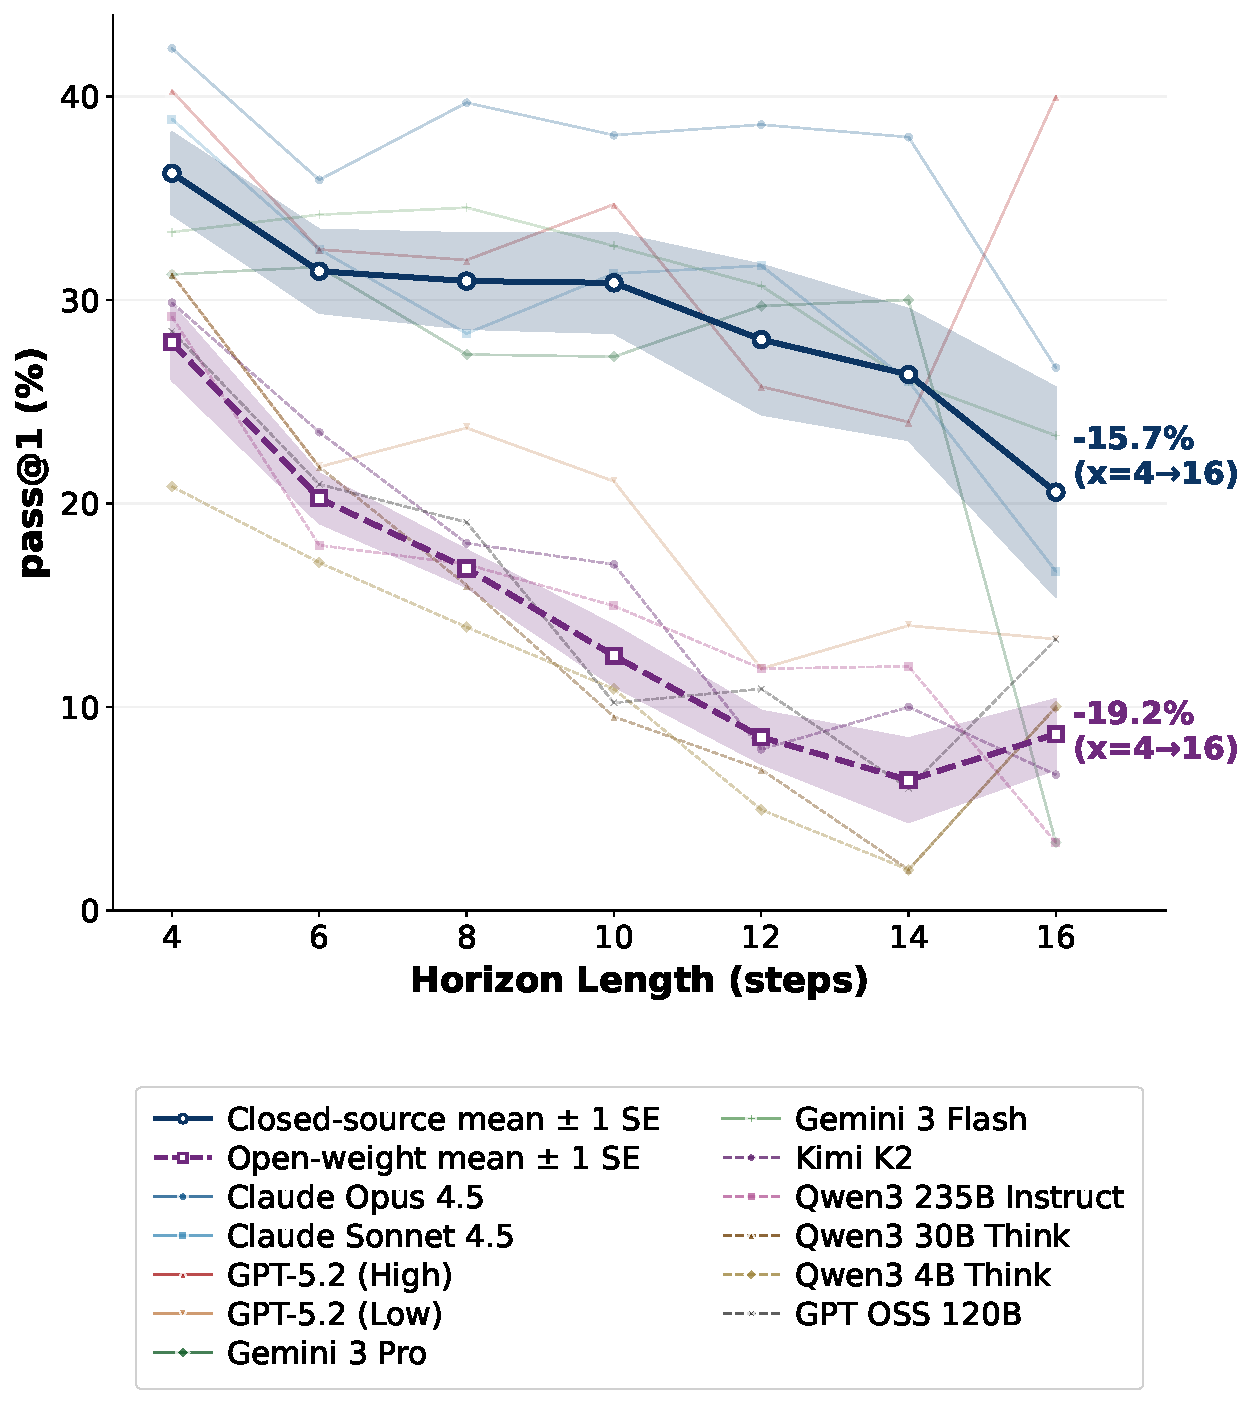
\includegraphics[width=1.0\linewidth]{figures/horizon_trend_single.pdf}
 \caption{\textbf{Performance degrades consistently with planning horizon.}
Pass@1 accuracy for closed-source (solid) and open-weight (dashed) models
across horizon lengths 4–16. Thick lines show the group mean $\pm$1 SE.
We observe monotonic degradation of performance for both sets, while open model performance falls more sharply with horizon length.}
 \label{fig:performance_by_horizon}
\end{figure}

\begin{figure*}[t]
 \centering
 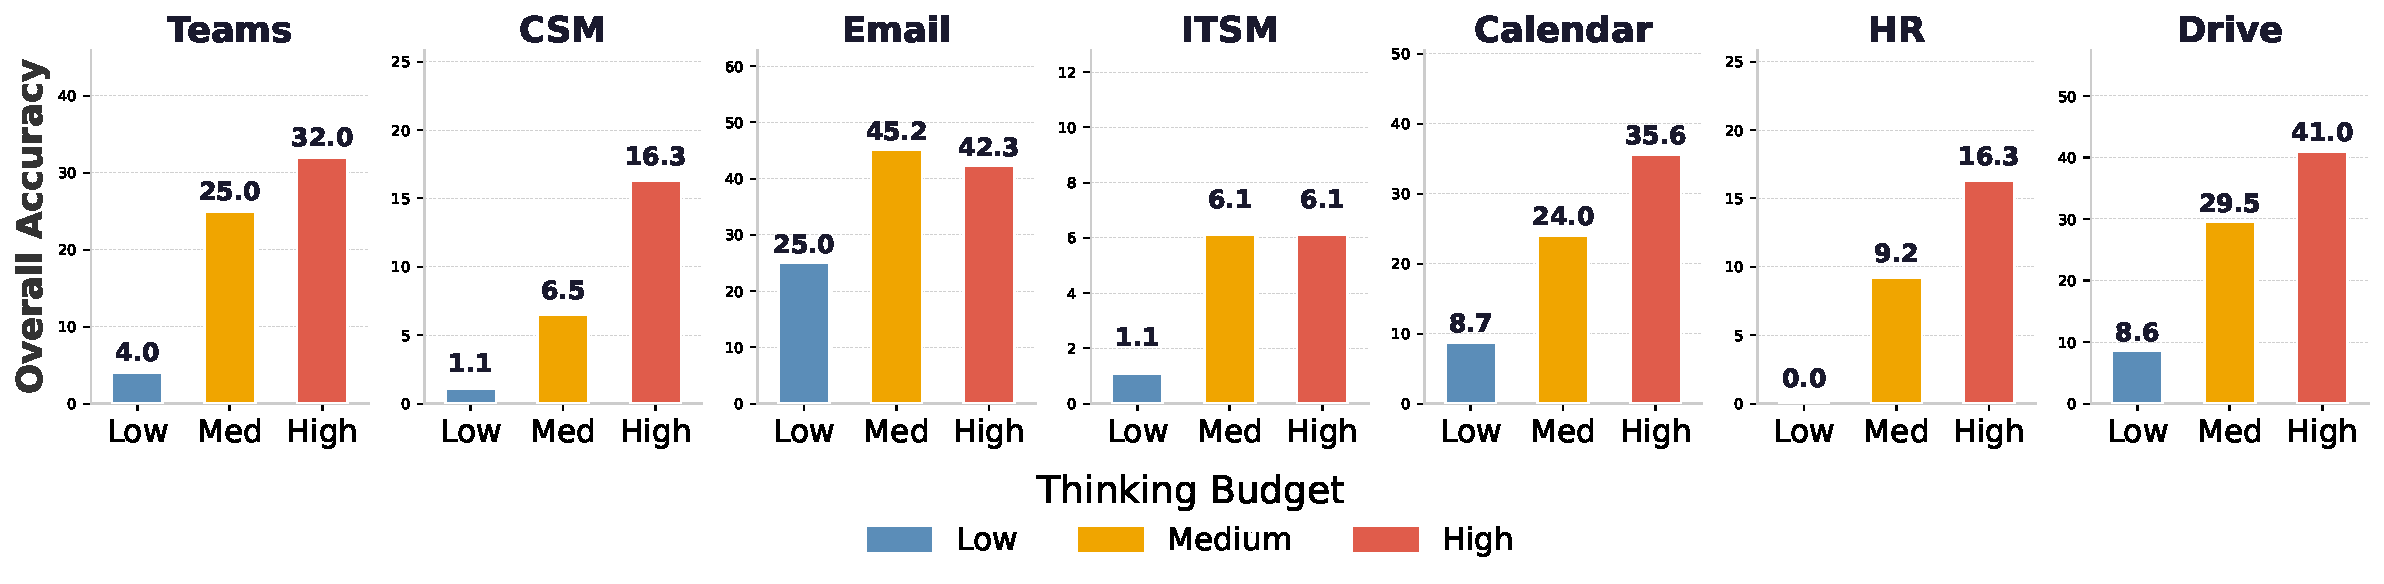
\includegraphics[width=1.0\linewidth]{figures/OSS-Thinking-Performance_pass1.pdf}
 \caption{\textbf{Impact of thinking budget on performance}
Histograms show the performance numbers with thinking budget with GPT-OSS-120B model \citep{openai2025gptoss120bgptoss20bmodel} across domains. The results show that the model with \textit{low} thinking budget performing poorly with performance steadily increasing with thinking budget. }
 \label{fig:thinking_budget_ablation}
\end{figure*}

\paragraph{How does performance scale with task horizon?}
To understand how model capabilities degrade with task complexity, we stratify tasks by their expected horizon length, which is proportional to the number of tool execution steps in the human created execution trajectories. As illustrated in \Cref{fig:performance_by_horizon}, performance across all models exhibits a consistent decay as the task horizon increases, reflecting the cumulative difficulty of maintaining reasoning integrity over multi-step sequences. The closed-source group, led by Claude Opus 4.5, demonstrates greater resilience, maintaining a performance lead even as the group mean drops from approximately 35\% at 4 steps to under 20\% by step 16. In contrast, the open-source cohort shows a much steeper decline, with models like Kimi K2 and GPT OSS 120B converging toward a success rate near 10\% at the maximum horizon. This near-universal trend suggests that while current models can navigate short-to-medium sequences, the rapid accumulation of errors in long-horizon tasks remains a critical barrier to autonomous reliability in production environments.

\paragraph{How does thinking budget affect performance?}
We evaluated the impact of test-time compute by varying the thinking budget (\textit{low, medium, high}) for the GPT-OSS-120B model \citep{openai2025gptoss120bgptoss20bmodel}. Increasing the thinking budget yields substantial improvements in task completion across almost all domains (see Figure~\ref{fig:thinking_budget_ablation}). Operating at a \textit{low} thinking budget causes the model to struggle severely, achieving near-zero accuracy on complex service and people-facing domains such as CSM (1.1\%), ITSM (1.1\%), and HR (0.0\%). Scaling to a \textit{high} budget unlocks significant capabilities, driving dramatic absolute gains in Drive ($8.6 \to 41.0$\%), Calendar ($8.7 \to 35.6$\%), and Teams ($4.0 \to 32.0$\%). This strong dependence on test-time compute underscores that \ours{} tasks require complex reasoning and planning to execute. However, we also observe that performance scaling is not universally monotonic; for instance, performance on Email peaks at the \textit{medium} budget (45.2\%) before receding slightly, and ITSM plateaus early ($1.1 \to 6.1\% \to 6.1\%$). This suggests that simply allocating more thinking tokens cannot universally overcome fundamental capability bottlenecks in certain workflows.

\subsection{Further Analysis}

% Custom command for a subtle, smaller improvement value
\newcommand{\up}[1]{\textsubscript{\color{green!50!black}$\uparrow$#1\%}}

\begin{table}[ht]
\centering
\small
\begin{tabular}{@{} l l S[table-format=2.2] @{\,} l S[table-format=2.1] @{\,} l S[table-format=2.2] @{\,} l @{}}
\toprule
\textbf{Model} & \textbf{Plan} & \multicolumn{2}{c}{\textbf{CSM}} & \multicolumn{2}{c}{\textbf{ITSM}} & \multicolumn{2}{c}{\textbf{HR}} \\
\midrule
\multirow{2}{*}{Kimi-K2}   & CP & 19.6  & \up{12.5} & 18.1 & \up{5.9}  & 17.2 & \up{9.0} \\
                           & HP & 42.2  & \up{35.1} & 29.1 & \up{16.9} & 34.5 & \up{26.3} \\ 
\cmidrule(lr){1-8}
\multirow{2}{*}{Qwen3-30B} & CP & 15.2  & \up{9.8}  & 11.7 & \up{5.0}  & 17.9 & \up{10.3} \\
                           & HP & 33.9  & \up{28.5} & 20.9 & \up{14.2} & 33.2 & \up{25.6} \\ 
\cmidrule(lr){1-8}
\multirow{2}{*}{Qwen3-4B}  & CP & 16.8  & \up{13.0} & 12.2 & \up{6.6}  & 19.6 & \up{12.5} \\
                           & HP & 37.16 & \up{33.4} & 23.3 & \up{17.7} & 36.4 & \up{29.3} \\
\bottomrule
\end{tabular}
\caption{Plan-Conditioned Execution Baseline. Comparison of performance with Claude Plans (CP) vs. Human Plans (HP). Green values indicate \% improvement over the ReAct baseline from Table~\ref{tab:main_results}.}
\label{tab:plan_conditioned}
\end{table}

The results above show that performance degrades sharply with horizon length and that models struggle most with planning rather than execution. To understand this further, we run a series of controlled ablations that both decouple planning from execution and build increasingly complex multi-agent systems to test whether distributing cognitive load across specialized agents can recover performance that a single monolithic agent cannot achieve.

\textbf{Automated planning improves weaker models consistently.} We introduce a planner-executor baseline in which a dedicated planner agent, instantiated with Claude Sonnet 4.5, one of our best peforming model, generates a high-level plan reasoning over user intent, policy constraints, and potential side effects. A separate executor then carries out tool execution using the same ReAct loop as the single-agent baseline. We evaluate three weaker models (Kimi-K2, Qwen-30B, and Qwen-4B) on the three most challenging domains (CSM, ITSM, and HR). As shown in Table~\ref{tab:plan_conditioned}, performance improves consistently across all models and domains with gains of 6-13\% confirming that planning quality is a meaningful bottleneck even when the executor model is fixed. 

\begin{figure}[h!]
 \centering
 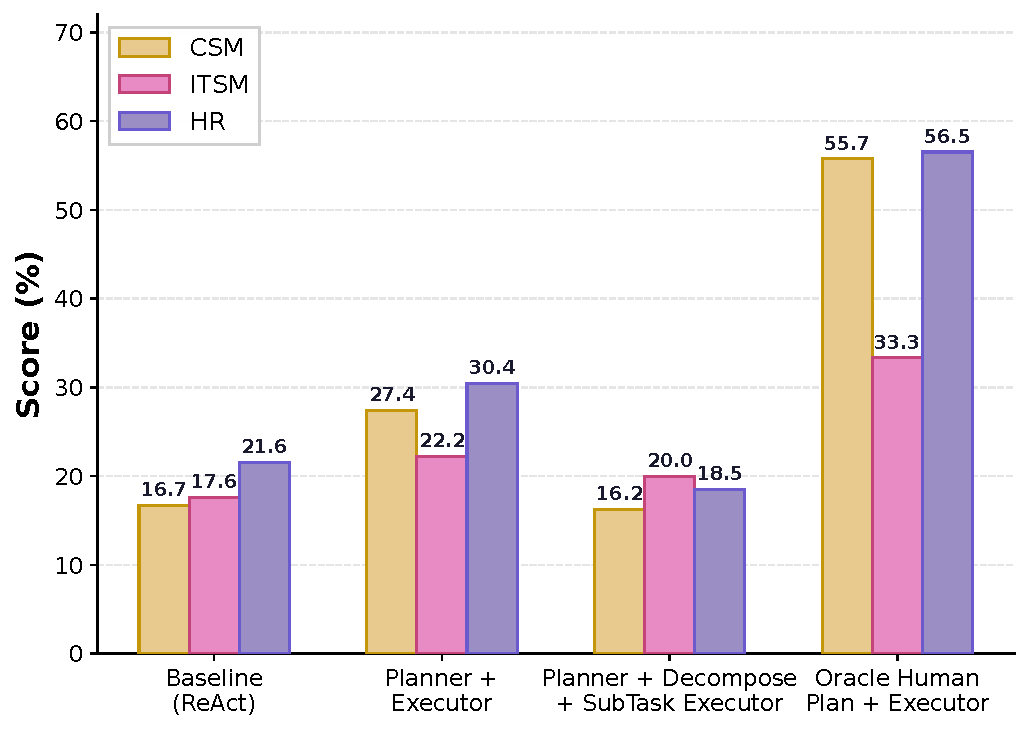
\includegraphics[width=1.0\linewidth]{figures/orchestrator_strategy_plot_overall.pdf}
 \caption{\textbf{ Impact of agentic orchestration on performance}
Histograms show the performance numbers with various multi-agentic architectures using Claude-Sonnet-4.5. The baseline is the simple ReAct loop described in Section~\ref{subsec:baselines}. \textit{Planner+Executor} architecture first prompts the model for a detailed plan, and performs a ReAct loop conditioned on the plan. \textit{Planner+Decompose+Subtask Executor} additionally does a task decomposition and calls subagents in a ReAct loop for each subtask. Finally, \textit{Oracle Human Plan + Executor} performs a ReAct execution loop conditioned on a human written plan.} 
 \label{fig:mas_orchestration_analysis}
\end{figure}

\textbf{Human-authored plans reveal a substantially higher ceiling.} To bound what better planning could achieve, we give the same executor models human-authored reference plans and ask them to carry out the corresponding tool execution, fully decoupling planning from execution. The gains are considerably larger than those from automated planning: 14-35 percentage points across models and domains, roughly doubling the improvements seen from Claude-generated plans. Notably, Qwen3-4B with human-authored plans (and Claude plans) is competitive with or outperforms larger models under the same condition. This suggests that when strategic reasoning is externalized, the primary remaining challenge is faithful instruction-following and precise tool invocation, both capabilities in which modern LLMs exhibit broad competence regardless of scale. This may also indicate that larger models, having stronger internal priors, are more prone to deviating from a provided plan, while smaller models tend to follow step-by-step instructions more literally---an advantage when those instructions are optimal. However, gap between the human plans and LLM plans indicates that current LLMs fall well short of human-level strategic reasoning on these tasks.

\textbf{More complex orchestration does not close this gap.} We evaluate two MAS configurations for Claude Sonnet 4.5: a \textit{Planner+Executor} system that conditions ReAct on an auto-generated plan, and a \textit{Planner+Decompose+Subtask Executor} system that additionally decomposes tasks and invokes a separate subagent per subtask. We evaluate these systems against the ReAct executor baseline with and without human authored plans. As shown in Figure~\ref{fig:mas_orchestration_analysis}, the \textit{Planner+Executor} setup consistently outperforms the ReAct baseline, yielding absolute gains of 10.7\% in CSM and 8.8\% in HR. However, the decomposition architecture is less robust. While it provides a minor lift in ITSM, it regresses in both CSM and HR, even falling below the base ReAct performance in CSM (16.2\% vs. 16.7\%). This is consistent with \ours{} tasks having strong sequential state dependencies that decomposition disrupts. Ultimately, the substantial remaining gap between automated systems and ReAct with human plans suggests that progress requires advances in constraint-aware plan generation rather than architectural complexity alone.

\paragraph{Failure Modes}
We performed a manual qualitative analysis of samples where models made partial progress but ultimately failed to complete the task. We observe several recurring failure patterns. Models frequently invoke tools that create database objects without first querying the necessary prerequisites, producing dangling records with broken foreign-key links \textbf{(Missing Prerequisite Lookup)}. For example, in a task requiring the creation of an HR topic under a specific category, the model skips retrieving available categories and inserts an orphaned record. Models also fail to trigger the follow-up actions mandated by system policies when certain state transitions occur \textbf{(Cascading State Propagation)}. Further failure modes include passing unverified identifiers to tool calls instead of resolving the correct IDs through prior tool interactions \textbf{(Incorrect ID Resolution)}, and prematurely declaring task completion before all required steps have been executed \textbf{(Premature Completion Hallucination)}. To futher systematically categorize these errors, we use an LLM (Claude Sonnet 4.5~\cite{claudeopus}) to tag the final-state SQL verifiers into three types based on their expert-written descriptions: i)~\textit{Task Completion} verifiers check whether the primary user objective was achieved; ii)~\textit{Integrity Constraints} verifiers check that the system remains in a consistent state with valid foreign-key relationships; and iii)~\textit{Permission and Process Compliance} verifiers check adherence to system policies governing permissions and procedural rules. Verifier pass rates for these categories are reported in \Cref{tab:verifier_analysis}. Models struggle most with \textit{Permission and Process Compliance}---a particularly critical gap for real-world deployment, where policy violations can cause cascading system failures and introduce serious security vulnerabilities. Refer to \Cref{app:errors} for examples of model failures.
